\sujet{Feature detector}
\index{Features:FAST corner detector}

\noindent
{\bf Duration: 1h30 / 20 points}

All documents allowed. NO internet connection, except for connection to campus website (to download the test images and to upload your results, and to use the different electronic documents).

\begin{wikipedia}

\begin{wrapfigure}{r}{40mm}\centering
 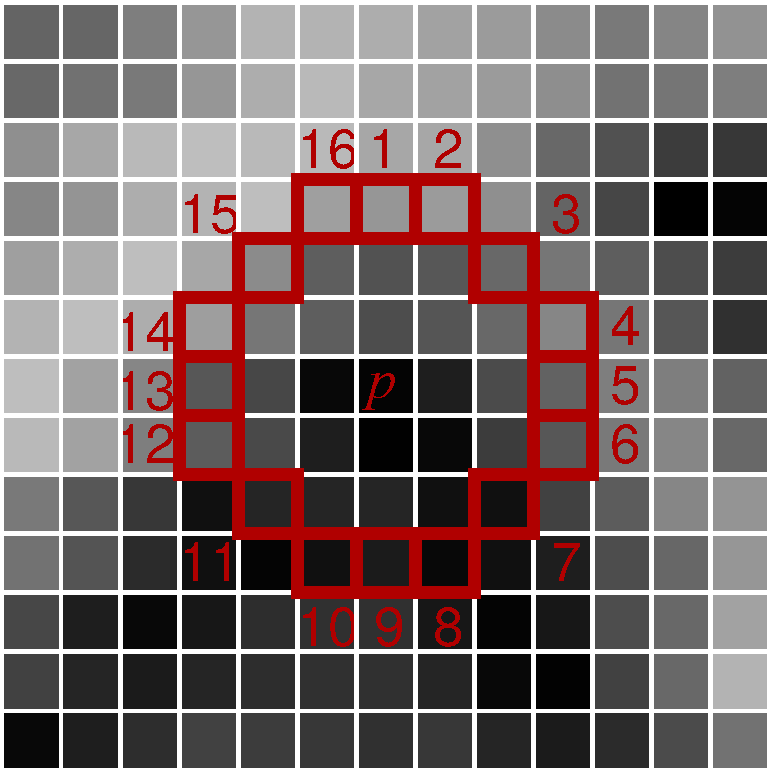
\includegraphics[width=\linewidth]{fast-corner2.pdf}
 \caption{Bresenham circle}
 \label{fig:exam:2018:ipr:bcircle}

\end{wrapfigure}
Features from accelerated segment test (FAST) is a corner detection method. FAST corner detector uses a circle of 16 pixels (a Bresenham circle of radius 3, see Fig.\ref{fig:exam:2018:ipr:bcircle}) to classify whether a candidate point p is actually a corner. Each pixel in the circle is labeled from integer number 1 to 16 clockwise. If a set of $N$ contiguous pixels in the circle are all brighter than the intensity of candidate pixel $p$ (denoted by $I_p$) plus a threshold value t or all darker than the intensity of candidate pixel $p$ minus threshold value $t$, then $p$ is classified as corner. The conditions can be written as:

\begin{enumerate}
   \item  Condition 1: A set of N contiguous pixels $S$, $\forall x \in S$, the intensity of x $(I_x) > I_p + t$
   \item  Condition 2: A set of N contiguous pixels $S$, $\forall x \in S$, $I_x < I_p - t$
    \end{enumerate}

So when either of the two conditions is met, candidate p can be classified as a corner. There is a tradeoff of choosing N, the number of contiguous pixels and the threshold value t. On one hand the number of detected corner points should not be too many, on the other hand, the high performance should not be achieved by sacrificing computational efficiency. N is usually chosen as 12.
\end{wikipedia}


\section{Counting the number of ones in an array (5 pts)}
\begin{qbox}
Given an array of 16 elements, code a function that returns the maximum number of adjacent ones. 
\begin{matlab}
function n = countContiguousOnes(x)
\end{matlab}
\end{qbox}

For example, if \minline{x=[1 1 1 0 0 1 1 1 1]}, then $n$ is equal to 7. 

\begin{mcomment}
\begin{mremark}
\begin{itemize}
 \item You can try to label the array and evaluate the area  of the considered regions.
 \item Use circshift in order to circularly shift the array and obtain the different configurations.
\end{itemize}

\end{mremark}
\end{mcomment}

\section{Access to elements in the Bresenham circle (5 pts)}
\index{Bresenham Circle}

The Bresenham circle is illustrated in Fig.\ref{fig:exam:2018:ipr:bcircle}.

 \begin{qbox}
  Code a function that extracts all values of the pixels at the coordinates given by the Bresenham circle from an array \minline{w} of size $7\times 7$.
  
  \begin{matlab}
   function x = fastPixels(w)
  \end{matlab}

 \end{qbox}


 \begin{mcomment}
\begin{mremark}
 Consider you want to extract the values of the 2D matrix A at coordinates (1,2) and (3,2), given as (row,col), at the same time. 
  Then, you would linearize your vector and compute A([4, 6]). Think of how to convert 2D coordinates into 1D coordinates. An example illustrates this property:
  \begin{matlab}
>> A =
     5     6     3
    10     3     6
     4     8     7

>> A(1,2)
ans =
     6

>> A(3,2)
ans =
     8
     
>> A([4, 6])
ans =
     6     8
\end{matlab}
 
 \end{mremark}
\end{mcomment}


\section{FAST corner detector (10 pts)}
The FAST corner detector checks every pixel (except border pixels, defined by the circle radius), evaluates the two conditions presented previously and decides if this is a corner or not, depending on the threshold value $t$ and the value $N$.

\begin{qbox}
\begin{itemize}
 \item 
 Code a matlab function that takes the image \minline{I} and outputs a binary image representing the corners as ones and the rest of the image as zeros.
 \item Test it on a small window.
 \item Test it on the wild roar image (see Fig.\ref{fig:exam:2018:ipr:examples}).
\end{itemize}

\end{qbox}

\begin{figure}
 \centering
 \subfloat[Original image.]{
\includegraphics[width=.45\linewidth]{sweden_road.png}}
 \hfill
 \subfloat[FAST corners, for $N=10$ and $t=0$.]{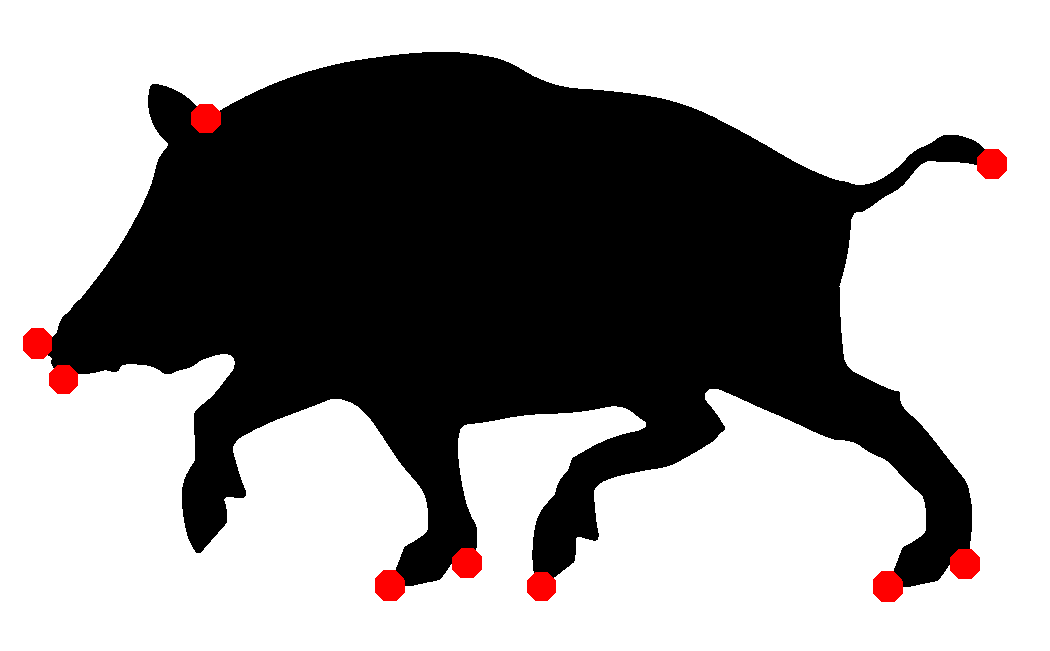
\includegraphics[width=.45\linewidth]{res_fast.png}}
 \caption{Application examples.}
 \label{fig:exam:2018:ipr:examples}
\end{figure}

